\section{Experiments}
\label{sec:experiments}

We evaluate the iterative fixed-point estimator on three dynamical systems that span the
identifiability spectrum predicted a priori by the observability analysis of
Section~\ref{sec:identifiability}: the epidemiological SIR model (structurally observable), the
ecological Lotka--Volterra model (observability matrix rank-deficient in one parameter direction),
and the physiological OGTT glucose--insulin model (weakly identifiable, with only the product
$mDI=S_I\sigma$ recoverable from glucose~\cite{ha2025disposition}). For each system we train the two networks $H_\phi,P_\psi$
by teacher forcing and compare the converged fixed point $\theta^*(\mathbf{x}_\mathrm{obs})$ against a
\emph{direct-regression baseline} --- a single network $x_\mathrm{obs}\mapsto\theta$ of matched
capacity trained by MSE on the identical data split. The comparison is diagnostic rather than
competitive: because both estimators minimize a squared loss, both are driven toward the conditional
mean (Proposition~\ref{prop:optimal_predictor}), so the baseline isolates the \emph{structural}
component of the error (Remark~\ref{rem:decomposition}(i)) from the iterative operator's own
approximation gap (ii).

\paragraph{Protocol.} Synthetic trajectories are generated by numerical integration under sparse,
partial observation (SIR/LV: $2\times10^4$ samples; OGTT: $5\times10^4$). Spectral normalization is
applied with a per-layer margin yielding a verified contraction constant
$\mathrm{Lip}_\mathcal{T}\approx 0.6<1$ (Section~\ref{subsec:sn}); inference uses $K=10$ fixed-point
iterations. We report coordinate-wise RMSE (physical units) and Pearson correlation $r$ between true
and predicted parameters; because RMSE is scale-dependent across systems, $r$ is the primary
scale-invariant indicator of whether a parameter is recovered at all.

\begin{table}[t]
\centering
\caption{Parameter recovery (RMSE\,/\,Pearson $r$) on synthetic test data. The direct baseline
recovers structurally identifiable parameters nearly perfectly ($r\!\approx\!0.98$); it fails
exactly on the observability-predicted non-identifiable directions (LV $\beta$; OGTT
$S_I,\sigma$ individually). The iterative estimator converges but exhibits an additional
approximation gap even where the problem is identifiable (SIR).}
\label{tab:recovery}
\begin{tabular}{llcc}
\hline
System & Parameter & Iterative (RMSE\,/\,$r$) & Direct baseline (RMSE\,/\,$r$) \\
\hline
SIR       & $\beta$   & $0.108\,/\,0.66$ & $\mathbf{0.026\,/\,0.98}$ \\
(wide)    & $\gamma$  & $0.105\,/\,0.68$ & $\mathbf{0.055\,/\,0.92}$ \\
\hline
Lotka--   & $\alpha$  & $0.102\,/\,0.54$ & $\mathbf{0.014\,/\,0.99}$ \\
Volterra  & $\beta$   & $0.115\,/\,0.02$ & $0.113\,/\,0.22$ \\
          & $\delta$  & $0.089\,/\,0.84$ & $\mathbf{0.012\,/\,0.99}$ \\
          & $\gamma$  & $0.096\,/\,0.62$ & $\mathbf{0.020\,/\,0.99}$ \\
\hline
OGTT      & $S_I$     & $0.265\,/\,0.65$ & $0.212\,/\,0.76$ \\
          & $\sigma$  & $0.338\,/\,0.65$ & $0.254\,/\,0.82$ \\
\hline
\end{tabular}
\end{table}

Table~\ref{tab:recovery} summarizes all runs; the following subsections read it through the theory.

\subsection{SIR: an identifiability control that isolates the operator gap}
\label{subsec:exp-sir}

The augmented SIR system satisfies the observability rank condition from its sparse partial
observations of $S(t)$ (Section~\ref{sec:identifiability}), so the conditional variance
$\operatorname{Var}(\theta\mid\mathbf{x}_\mathrm{obs})$ is negligible and the structural term
(Remark~\ref{rem:decomposition}(i)) vanishes. Consistently, the direct baseline recovers $(\beta,\gamma)$
almost exactly ($r=0.98,0.92$). The iterative estimator, although it converges to a unique fixed point
(Theorem~\ref{thm:contraction}), attains only $r=0.66,0.68$ (Figure~\ref{fig:sir-scatter}): predictions
concentrate in a narrow band and $\mathcal{R}_0$ saturates. Since the problem is identifiable, this
residual bias cannot be structural; it is precisely the operator-approximation term
(Remark~\ref{rem:decomposition}(ii)) --- the composition $P_\psi\!\circ\!H_\phi$ does not preserve
$\theta$ perfectly, keeping the one-step residual $\varepsilon(\mathbf{x}_\mathrm{obs})$ bounded away from
zero. SIR thus serves as a control that exhibits (ii) in isolation, and cautions against reading the
iterative estimator's accuracy as evidence about identifiability. This gap is exactly the cost of the
reconstruction detour identified in Proposition~\ref{prop:ceiling}: the direct regressor, which maps
$\mathbf{x}_\mathrm{obs}$ to $\theta$ without reconstructing the hidden state, reaches the
conditional-mean ceiling far more closely ($r\approx0.98$) than the iteration ($r\approx0.66$), on the
identical data. (The same picture holds on a narrow-range variant matching commonly reported values,
where the baseline reaches $r\approx0.99$ and the iteration $r\approx0.4$--$0.5$.)

To confirm that the gap is driven by the difficulty of reconstructing the hidden state --- and not by
non-identifiability --- we sweep the observation density (Figure~\ref{fig:sir-density}). As the number
of observation points increases from $4$ to $30$, the iterative estimator's recovery improves
monotonically ($r_\beta: 0.66\!\to\!0.71\!\to\!0.75\!\to\!0.78$): denser observations make the hidden
trajectory easier to reconstruct, shrinking $\varepsilon$ and, by Lemma~\ref{lem:error_bound}, the
fixed-point error. This validates the correctness bound as non-vacuous. Yet the improvement plateaus
well below the direct-regressor ceiling ($r\approx0.98$, already at $4$ points), consistent with
Proposition~\ref{prop:ceiling}: the reconstruction detour retains a residual cost that observation
density alone does not remove. Correctness is approached, but not achieved, precisely in the regime
--- dense, well-conditioned observation --- that the sparse-and-partial premise of this paper excludes.

\begin{figure}[t]
\centering
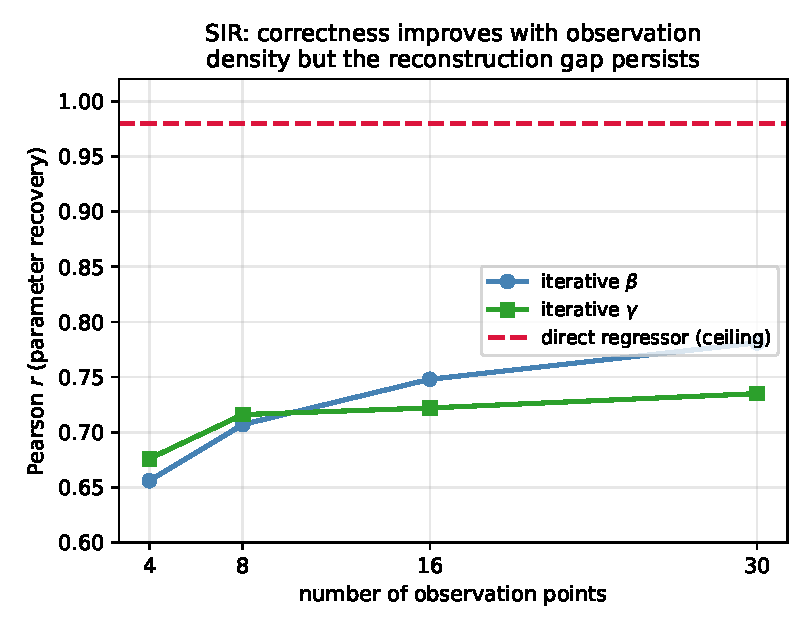
\includegraphics[width=0.6\linewidth]{figures/exp/sir_density_sweep.pdf}
\caption{SIR observation-density sweep (identifiable regime, unknown-hidden-state setting). The
iterative estimator's parameter recovery improves monotonically with the number of observation points
--- validating that the fixed-point error is governed by the one-step residual
(Lemma~\ref{lem:error_bound}) --- but plateaus below the direct-regressor ceiling
(Proposition~\ref{prop:ceiling}): denser data eases hidden-state reconstruction yet does not remove the
detour cost.}
\label{fig:sir-density}
\end{figure}

\begin{figure}[t]
\centering
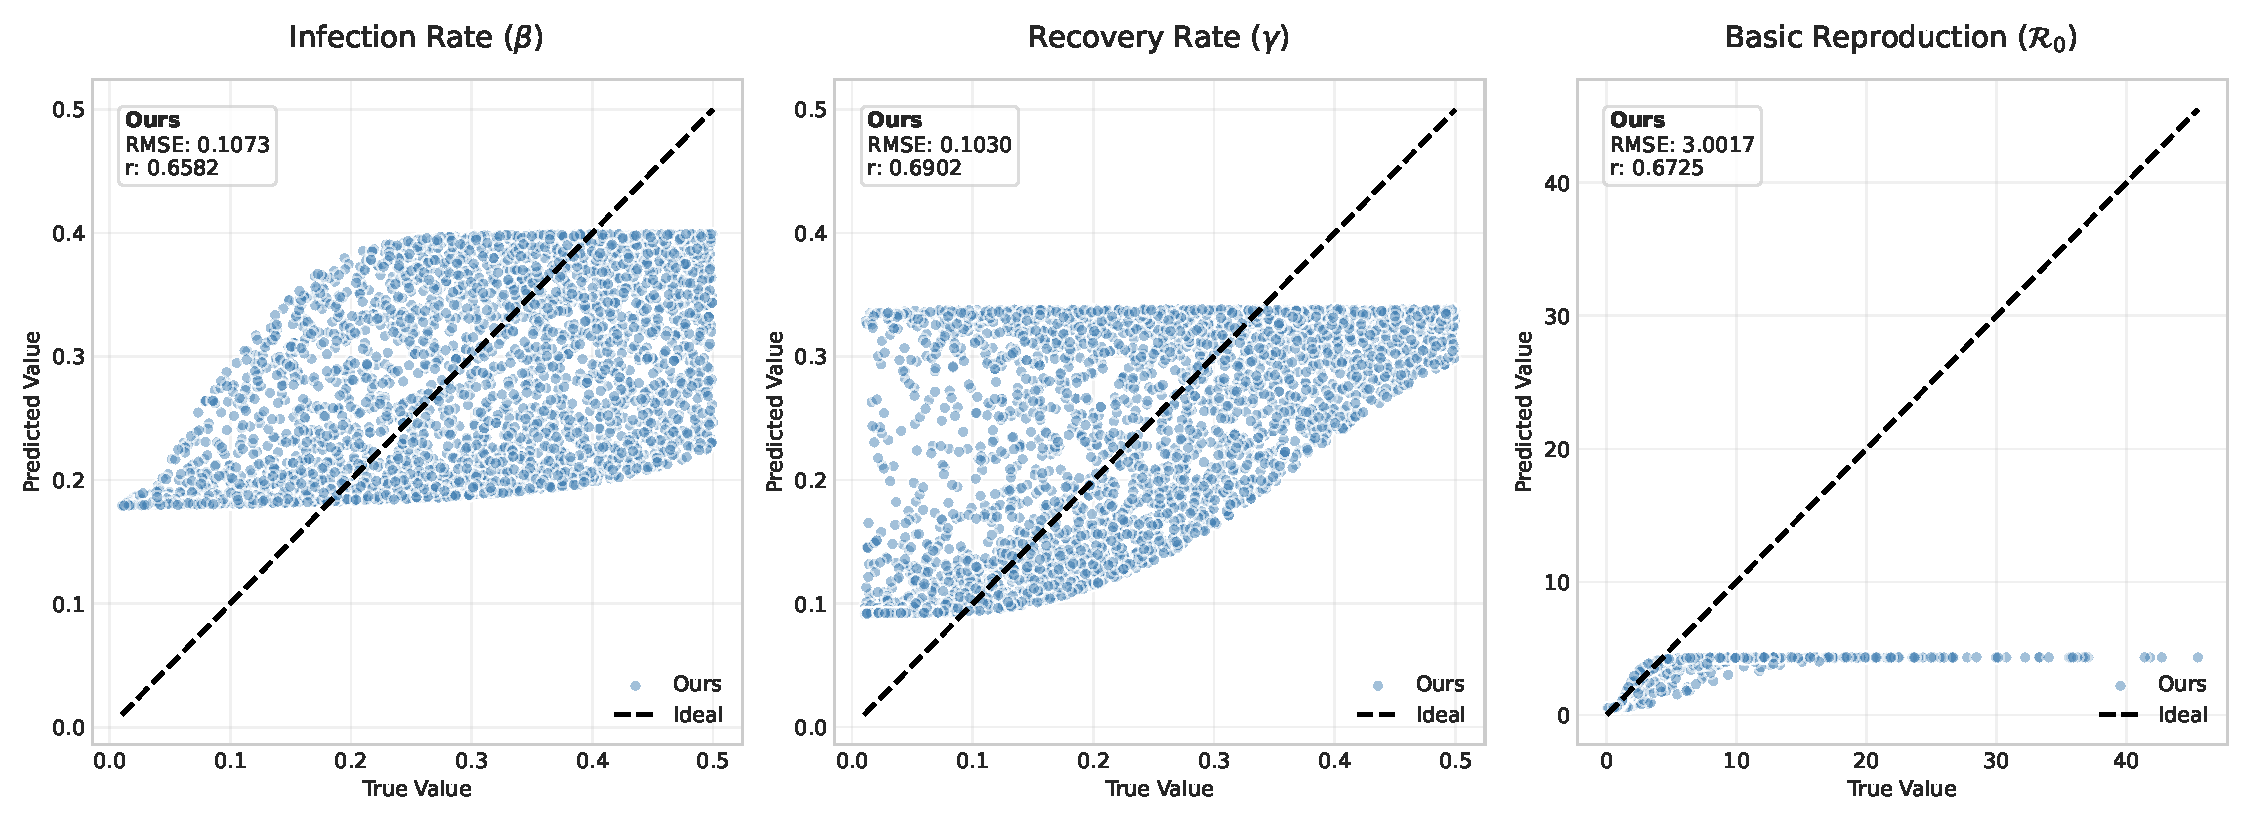
\includegraphics[width=0.92\linewidth]{figures/exp/sir_scatter_wide_iter.pdf}
\caption{SIR parameter recovery, iterative estimator. Predictions (blue) versus ground truth for
$\beta,\gamma,\mathcal{R}_0$. Despite guaranteed convergence, predictions compress toward a central
band and $\mathcal{R}_0$ saturates --- the operator-approximation gap of
Remark~\ref{rem:decomposition}(ii), present even though SIR is identifiable (cf. the direct baseline,
$r\approx0.98$).}
\label{fig:sir-scatter}
\end{figure}

\subsection{Lotka--Volterra: observability predicts which parameters are recoverable}
\label{subsec:exp-lv}

For prey-only observation the augmented Lotka--Volterra observability matrix is rank-deficient
($\operatorname{rank}\mathbf{O}=5<6$; Section~\ref{sec:identifiability}), and the deficient direction
corresponds to the interaction parameter $\beta$. The experiment confirms this prediction sharply: the
direct baseline recovers $\alpha,\delta,\gamma$ nearly perfectly ($r=0.99,0.99,0.99$) but collapses on
$\beta$ ($r=0.22$), while every other coordinate remains recoverable (Figure~\ref{fig:lv-scatter}).
Thus the a-priori observability rank predicts, parameter by parameter, exactly where estimation is
possible --- turning ``the method sometimes fails'' into a quantitative statement about the problem.
The iterative estimator recovers the same identifiable coordinates with the additional bias of
(ii) ($r=0.54$--$0.84$) and, like the baseline, cannot recover the unobservable $\beta$.

\begin{figure}[t]
\centering
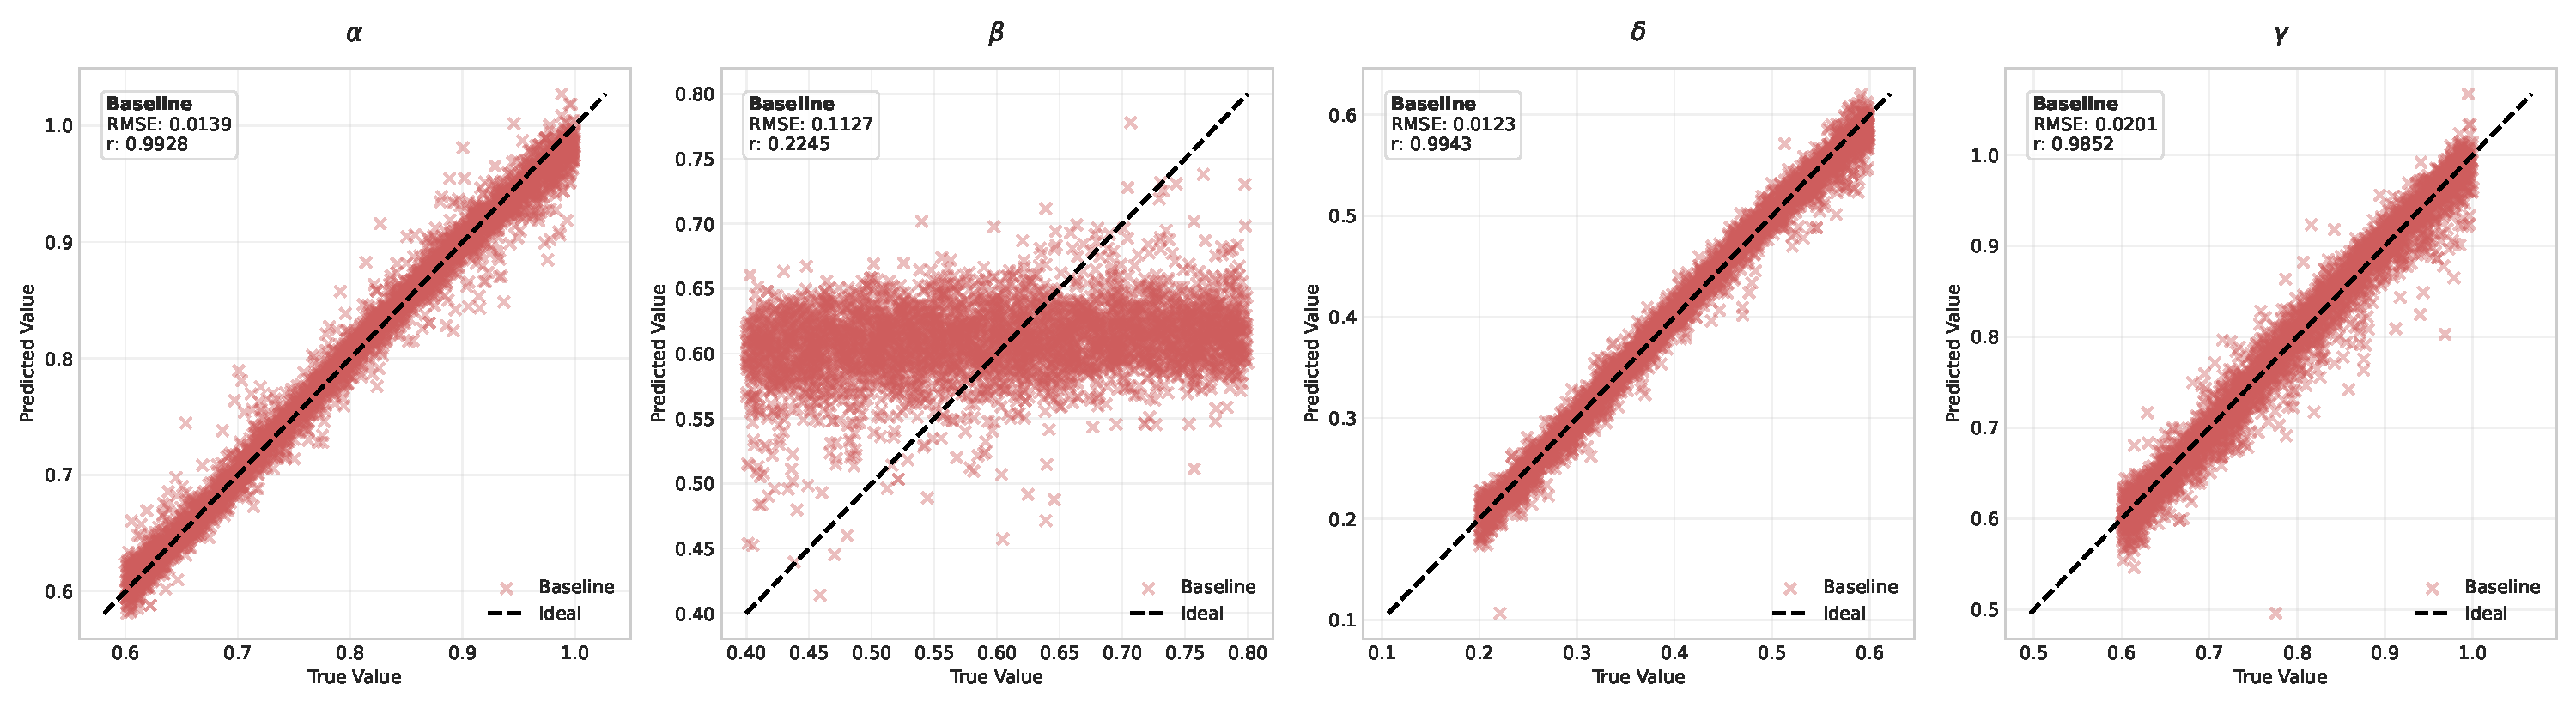
\includegraphics[width=0.92\linewidth]{figures/exp/lv_scatter_base.pdf}
\caption{Lotka--Volterra recovery, direct baseline. Three parameters are recovered nearly perfectly
($\alpha,\delta,\gamma$: $r\approx0.99$); the interaction parameter $\beta$ is not
($r=0.22$)---exactly the direction the observability matrix flags as rank-deficient
(Section~\ref{sec:identifiability}).}
\label{fig:lv-scatter}
\end{figure}

\subsection{OGTT: structural collapse onto an off-fiber locus}
\label{subsec:exp-ogtt}

Under glucose-only observation, $\theta=(S_I,\sigma)$ is identifiable only through the product
$mDI=S_I\sigma$ (Section~\ref{sec:identifiability}); the conditional distribution along each fiber
$\{S_I\sigma=c\}$ is non-degenerate, so the structural term (i) dominates. This is the regime targeted
by Corollary~\ref{cor:lower_bound} and Proposition~\ref{prop:off_fiber}.

Figure~\ref{fig:ogtt-collapse} makes the predicted behavior visible. \emph{(Left)} the joint
distribution of predictions collapses from the two-dimensional ground-truth cloud onto an essentially
one-dimensional locus --- the joint-distribution collapse of Corollary~\ref{cor:lower_bound}.
\emph{(Center)} the identifiable product $\log(S_I\sigma)$ (the ``stiff'' direction) is recovered, its
density matching the ground truth (Pearson $r=0.93$ for the iterative estimator, $r=0.99$ for the
baseline). \emph{(Right)} the two individual coordinates are \emph{both} unrecovered, and to the same
degree: $r(S_I)=r(\sigma)=0.65$ for the iterative estimator and $r(S_I)=0.76,\ r(\sigma)=0.82$ for the
baseline. Neither coordinate is privileged --- only the product is pinned down, while the estimate is
free to slide along the fiber. The signature predicted by Corollary~\ref{cor:off_fiber_product} ---
that the recovered product is biased relative to the true identifiable statistic and the estimate
leaves the physical fiber --- is directly observed. Crucially, the direct baseline exhibits the
\emph{same} structural collapse (it too recovers the product but not the individual coordinates),
confirming that the limitation binds any squared-loss point estimator and is not an artifact of the
fixed-point iteration.

\begin{figure}[t]
\centering
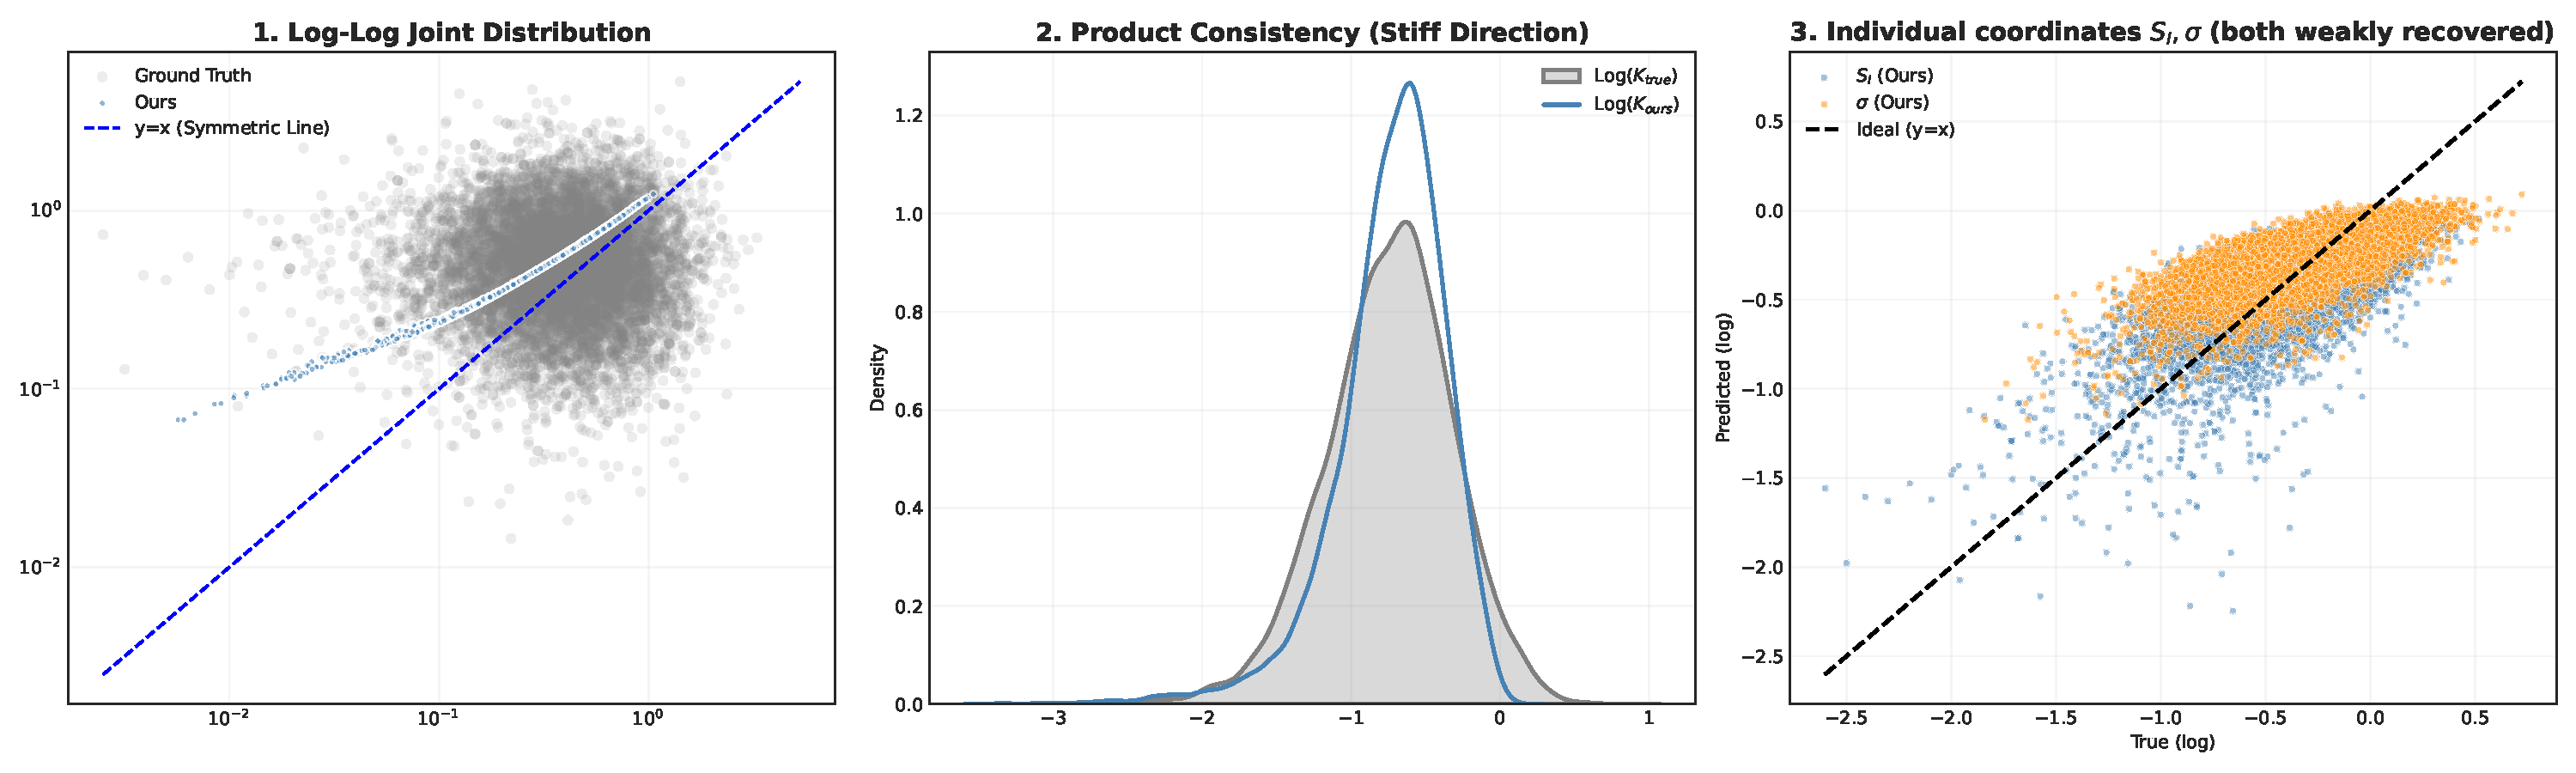
\includegraphics[width=\linewidth]{figures/exp/ogtt_collapse_iter.pdf}
\caption{OGTT joint-distribution collapse (iterative estimator; the direct baseline is
qualitatively identical). \emph{Left:} predictions (blue) collapse the 2-D ground-truth cloud (grey)
onto a 1-D locus. \emph{Center:} the identifiable product $S_I\sigma$ (stiff direction) is recovered
($r=0.93$). \emph{Right:} the two individual coordinates $S_I$ and $\sigma$ are both unrecovered and to
the same degree ($r=0.65$ each), neither privileged --- the estimate slides freely along the fiber.
This realizes the regression-to-mean of Corollary~\ref{cor:lower_bound} and the off-fiber conditional
mean of Proposition~\ref{prop:off_fiber} / Corollary~\ref{cor:off_fiber_product}.}
\label{fig:ogtt-collapse}
\end{figure}

\subsection{Convergence and the role of the contraction margin}
\label{subsec:exp-convergence}

Figure~\ref{fig:ogtt-phase} visualizes the fixed-point dynamics in the $(S_I,\sigma)$ plane:
trajectories launched from widely separated initializations all converge to a \emph{single} fixed
point (Theorem~\ref{thm:contraction}), yet that fixed point does not coincide with the ground truth ---
a direct picture of ``convergence $\neq$ correctness.'' The annotated one-step residual
$\varepsilon=0.08$ and fixed-point error $\|\theta^*-\theta^{\mathrm{true}}\|=0.11$ are consistent with
the bound $\varepsilon/(1-\mathrm{Lip}_\mathcal{T})$ of Lemma~\ref{lem:error_bound}.

Finally, we vary the spectral-normalization margin. Across per-layer targets giving verified
contraction constants $\mathrm{Lip}_\mathcal{T}\in\{0.28,0.60,0.89,0.92\}$, parameter accuracy is
essentially flat (SIR $\beta$: RMSE $0.11$--$0.11$, $r\approx0.64$--$0.68$); without spectral
normalization the composite Lipschitz constant is $\gg 1$, the iteration fails to contract, and
accuracy collapses ($r<0$). This matches the theory: spectral normalization supplies the convergence
\emph{guarantee}, but within the contractive regime the residual error is set by
$\varepsilon(\mathbf{x}_\mathrm{obs})$ --- the structural and operator terms of
Remark~\ref{rem:decomposition} --- not by the size of the margin.

\begin{figure}[t]
\centering
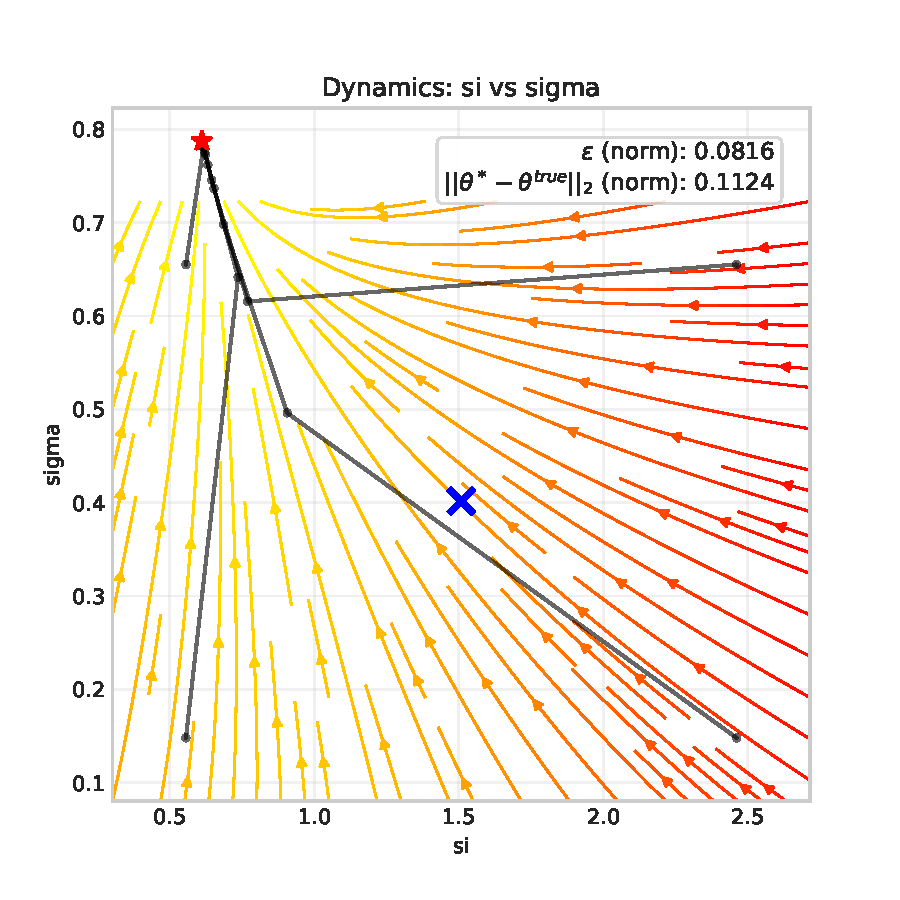
\includegraphics[width=0.62\linewidth]{figures/exp/ogtt_phase.pdf}
\caption{Fixed-point dynamics for OGTT in the $(S_I,\sigma)$ plane. Trajectories from four
initializations converge to one fixed point (red star), which differs from the ground truth (blue
cross): convergence does not imply correctness. Annotations report the one-step residual $\varepsilon$
and the fixed-point error, consistent with Lemma~\ref{lem:error_bound}.}
\label{fig:ogtt-phase}
\end{figure}

\paragraph{A note on distribution shift.} On real clinical OGTT measurements (out of the synthetic
training distribution), the direct baseline's predictions diverge under denormalization, whereas the
iterative estimator's strongly biased output remains bounded. We record this as an observation about
the two estimators' behavior under distribution shift; a robustness claim is beyond the scope of the
present, characterization-focused study.